\chapter{Numerical Algorithms}\label{sec:numerics}

The system of equations is written as
\begin{equation}
  \frac{\partial \boldsymbol{q}}{\partial t} = \boldsymbol{f}_q(\boldsymbol{q},
  \boldsymbol{s},t) \;,\qquad
  \frac{\partial \boldsymbol{s}}{\partial t} = \boldsymbol{f}_s(\boldsymbol{q},
  \boldsymbol{s},t) \;,
\label{equ:problem}
\end{equation}
where $\boldsymbol{q}$ and $\boldsymbol{s}$ are the flow and scalar
vectors. For the compressible formulation,
\begin{equation}
  \boldsymbol{q} = (\rho, \rho u_1, \rho u_2, \rho u_3, \rho e)^T \;,\qquad
  \boldsymbol{s} = (\rho s_1, \rho s_2, \ldots)^T \;,
\end{equation}
and $\boldsymbol{f}_q$ and $\boldsymbol{f}_s$ are the corresponding
right-hand side of the equations. The energy equation can be also solved in
terms of the total energy per unit volume $\rho(e+v^2/2)$ instead of the
internal energy per unit volume $\rho e$. If the incompressible equations are
solved, then 
\begin{equation}
  \boldsymbol{q} = (u_1, u_2, u_3)^T \;,\qquad
  \boldsymbol{s} = ( s_1, s_2, \ldots)^T \;.
\end{equation}

The basic formulation is the method of lines, so that the algorithm is a
combination of different spatial operators needed to calculate the right-hand
side of the equations (typically, derivatives) and a time marching scheme. An
implicit treatment of the diffusive terms in the incompressible case has also
been implemented.

%%%%%%%%%%%%%%%%%%%%%%%%%%%%%%%%%%%%%%%%%%%%%%%%%%%%%%%%%%%%%%%%%%%%%%%%%%%%%%%%
%%%%%%%%%%%%%%%%%%%%%%%%%%%%%%%%%%%%%%%%%%%%%%%%%%%%%%%%%%%%%%%%%%%%%%%%%%%%%%%%
\section{Spatial operators}

Spatial operators are based on finite difference methods (FDM). There are two
levels of operator routines. The low-level libraries contains the basic
algorithms and is explained in this section. It consists of the FDM kernel
library {\tt fdm} and three-dimensional operators in the {\tt operators}
library. (The latter is still part of the general {\tt dns} library but it
should be migrated into its own {\tt operators} library. The file name starts,
generally, with {\tt opr\_}.) The high-level library {\tt fields} is composed of
routines that are just a combination of the low-level routines.

\subsection{Derivatives}\label{sec:fdm}

Spatial derivatives are calculated using fourth- or sixth-order compact Pad\'{e}
schemes as described by \cite{Lele:1992} and extended by \cite{Shukla:2005} for
non-uniform grids. The routines {\tt PARTIAL\_X}, {\tt PARTIAL\_Y} and {\tt
  PARTIAL\_Z}, and correspondingly {\tt PARTIAL\_XX}, {\tt PARTIAL\_YY} and {\tt
  PARTIAL\_ZZ} manage these operations. The kernels of the specific algorithms
are in the library {\tt fdm}.

We restrict ourselves to the 5-point stencils
\begin{equation}
a_{-1}s'_{j-1}+a_{0}s'_{j}+a_{+1}s'_{j+1}=
\frac{1}{h}(b_{-2}s_{j-2}+b_{-1}s_{j-1}+b_{0}s_{j}+b_{+1}s_{j+1}+b_{+2}s_{j+2}) \;,
\label{equ:coefs}
\end{equation}
and similarly for the second-order derivative, where the components of the
$n$-dimensional vectors $\mathbf{s}=(s_j)$, $\mathbf{s'}=\delta_x
\mathbf{s}=(s'_j)$ and $\mathbf{s''}=\delta_{xx} \mathbf{s}=(s'_j)$ are,
respectively, approximations to the values $\{s(x_j):\, j=1,\ldots,n\}$ of a
function $s(\cdot)$ defined on a finite interval $[x_1\,,x_n]$ and its first-
and second-order derivatives evaluated at those same points $\{x_j\}$. The
coefficients for the first-order derivative are given in
table~\ref{tab:coeffs}. Global schemes are constructed as a combination of $n$ of
these formulae, using biased finite differences at the boundaries in case of
non-periodicity.  We define the global algorithm (35653) by using the centered
scheme C6 at the $(n-4)$ interior points, and the biased schemes B5 at $j=2$ and
B3 at $j=1$ with the corresponding symmetric counterpart at $j=n-1$ and $j=n$,
respectively \cite{Carpenter:1993}. Those global schemes can be represented as
\begin{equation}
  A_1\, \delta_x \mathbf{s}=(1/h)B_1\, \mathbf{s} \;, \qquad
  A_2\, \delta_{xx} \mathbf{s}=(1/h^2)B_2\, \mathbf{s}
\label{equ:fdm}
\end{equation}
where $h=(x_n-x_1)/(n-1)$ is a reference space step and the square matrices
$A=(a_{ij})$ and $B=(b_{ij})$ are narrow banded, namely, tri-diagonal and
penta-diagonal, respectively. (At the boundary points, 1 or 2 additional points
in the right-hand sides can be used to increase the order, which in theory
increases the bandwidth of the matrices. However, it can be handled locally
without a penalty in memory requirements nor computational time.)  If periodic
boundary conditions are used, these are imposed at $x_{n+1}$ and not at $x_n$,
i.e.  $s(x_{n+1})=s(x_1)$. The size of the domain is then
$L=n(x_n-x_1)/(n-1)=nh$ instead of $x_n-x_1=(n-1)h$, and we do not save the
information at $x_{n+1}$. The matrices $A$ and $B$ are then circulant instead of
banded.  In any of both cases, standard Thomas' algorithm is used to solve those
linear systems efficiently. In particular, an LU decomposition is performed
during the initialization and equations can be normalized such that the
right-hand side contains always at least one diagonal of just ones, so as to
save memory and computational time (see routine {\tt
  fdm\_initialize}). Conceptually, it is sometimes advantageous to think about
equation~(\ref{equ:fdm}) as the definition of linear finite-difference operators
$\delta_x: \mathbb{R}^n \rightarrow \mathbb{R}^n$, $\mathbf{s'} = \delta_x\mathbf{s} =
(1/h)(A_1^{-1}B_1)\mathbf{s}$, and $\delta_{xx}: \mathbb{R}^n \rightarrow \mathbb{R}^n$,
$\mathbf{s''} = \delta_{xx}\mathbf{s} = (1/h^2)(A_2^{-1}B_2)\mathbf{s}$. Then,
we can use some results from linear algebra \citep{Mellado:2012}.

\begin{table}[!ht]
\centering
\begin{tabular}{l@{\hspace{6ex}}ccc@{\hspace{6ex}}ccccc@{\hspace{6ex}}c}\hline
&$a_{-1}$&$a_{0}$&$a_{+1}$&$b_{-2}$&$b_{-1}$&$b_{0}$&$b_{+1}$&$b_{+2}$&$t$\\ \hline 
C2&0        &1&0       & 0 & $^{-1}\!/\!_2$ & 0 &$^1\!/\!_2$ & 0&
$\;\,^{1}\!/\!_{3!}\,h^2s^{(3)}$\\
C4&$^1\!/\!_4$&1&$^1\!/\!_4$& 0 &$ ^{-3}\!/\!_4$ & 0 &$^3\!/\!_4$ & 0&
$^{-1}\!/\!_{5!}\,h^4s^{(5)}$\\
C6&$^1\!/\!_3$&1&$^1\!/\!_3$&$ ^{-1}\!/\!_{36}$ &$ ^{-7}\!/\!_9$  & 0 &
$^7\!/\!_9$  &$^{1}\!/\!_{36}$&
$\;\,^{4}\!/\!_{7!}\,h^6s^{(7)}$\\
B1&0      &1&0       & 0 & 0 & -1 & 1 & 0&
$\;\,^{1}\!/\!_{2!}\,h\;\,s^{(2)}$\\
B3&0      &1&2       & 0 & 0 & $^{-5}\!/\!_2$ & 2 &$ ^1\!/\!_2$&
$^{-2}\!/\!_{4!}\,h^3s^{(4)}$\\
B5&$^1\!/\!_6$&1&$^1\!/\!_2$& 0 &$ ^{-10}\!/\!_{18}$ &$ ^{-1}\!/\!_2$ & 1&
$^{1}\!/\!_{18}$&$^{-2}\!/\!_{6!}\,h^5s^{(6)}$\\\hline
\end{tabular}
\caption{Coefficients of the finite-difference formulae (\ref{equ:coefs}).
  The first three rows are centered differences, the last three are biased
  differences. The matrix $A_1$ in (\ref{equ:fdm}) is constructed in terms of
  the coefficients $\{a_i\}$, the matrix $B_1$ in terms of $\{b_i\}$. The last
  column contains the leading order term of the local truncation error defined
  by (\ref{equ:truncation1}).}
\label{tab:coeffs}
\end{table}

The local truncation error of the FDM approximation to the first-order
derivative in~(\ref{equ:fdm}) is defined by
\begin{equation}
\mathbf{t_1}=
\frac{1}{h}B_1\left(\begin{array}{c}s(x_1)\\\vdots\\s(x_n)\end{array}\right)-
A_1\left(
\begin{array}{c}\frac{ds}{dx}(x_1)\\\vdots\\\frac{ds}{dx}(x_n) 
\end{array}\right)\;,
\label{equ:truncation1}
\end{equation}
which yields $\boldsymbol{\epsilon} = -A_1^{-1}\mathbf{t}$ as the discretization
errors $\{\epsilon_j=ds/dx(x_j)-s'_j\,:\;j=1,\ldots,n\}$. The explicit
expression for the components of $\mathbf{t}$ can be found in
table~\ref{tab:coeffs}. Similarly for the second-order derivative, vector
$\mathbf{t_2}$ (to be written).

For notational convenience in the following discussion on Fourier analysis, we
change the index so that it varies between $j=0$ and $j=n-1$. We can define a
new sequence of numbers $\{\hat{s}_k\}_0^{n-1}$ from $\{s_j\}_0^{n-1}$ by
\begin{equation}
\hat{s}_k=\frac{1}{n}\sum_0^{n-1}s_j\exp(-i\omega_kj)\;,\qquad
s_j=\sum_0^{n-1}\hat{s}_k\exp(i\omega_kj)\;,
\label{equ:dft}
\end{equation}
where $\{\omega_k=(2\pi/n)k:\, k = 0,\ldots,n-1\}$ is the scaled wavenumber and
$i=\sqrt{-1}$ is the imaginary unit. We use the library FFTW in the code for
this transformation~\footnote{visit {http://www.fftw.org/}}. Note that
$\hat{s}_{k+n}=\hat{s}_k$ because $\exp(-i2\pi j)=1$ for any integer number $j$,
so that we can write
\begin{equation}
  s_j =  \sum_{-n/2+1}^{n/2} \hat{s}_k \exp[i\omega_kj]\;.  
\end{equation}
The expression above coincides with the Fourier series $\sum_{-n/2}^{n/2}
\hat{s}_k \exp[i\kappa_kx]$ of the function $s(x)$ over the interval $[0,L]$
particularized at the grid points $\{x_n\}$ provided that the spectral content
of the function $s(x)$ beyond the Nyquist frequency
$\kappa_{n/2}=(2\pi/L)(n/2)=2\pi/(2h)=\pi/h$ is zero. Then we have the relation
$\kappa_kh=\omega_k$ between the wavenumber $\kappa_k=(2\pi/L)k$ and the scaled
wavenumber $\omega_k$. In principle, both $\{\hat{s}_k\}$ from $\{s_j\}$ are
complex numbers; however, the sequence $\{\hat{s}_k\}$ is typically real and we
only need to know the Fourier modes between $k=0$, the mean value, and $k=n/2$,
the Nyquist frequency, because of the symmetry. Then, $\omega_k$ varies between
0 and $\pi$ and $\kappa_k$ varies between 0 and $\pi/h$. A third quantity
sometimes used in the discussion is the number of points per wavelength
$\mathrm{PPW}_k=(L/k)/h=2\pi/\omega_k$; for a given wavelength $L/k$, or
wavenumber $\kappa_k$, reducing the grid step $h$ and thus increasing resolution
-- increasing $\mathrm{PPW}_k$ -- means reducing the scaled wavenumber
$\omega_k$ towards zero.

The previous framework allows us to understand the FDM using the so-called von
Neumann analysis. We know that the exact values of $\{s'_j\}$ and $\{s''_j\}$
under the conditions stated above are
\begin{equation}
s'(x_j) =\sum_0^{n-1} (i\omega_k/h)  \hat{s}_k\exp(i\omega_kj)\;,\qquad 
s''(x_j)=\sum_0^{n-1} (-\omega^2_k/h^2)\hat{s}_k\exp(i\omega_kj)\;,
\end{equation}
having simply used the previous relation $\kappa_k=\omega_k/h$. The FDM
approximations can be written as
\begin{equation}
s'_j =\sum_0^{n-1} (\lambda_1/h)  \hat{s}_k\exp(i\omega_kj)\;,\qquad 
s''_j=\sum_0^{n-1} (\lambda_2/h^2)\hat{s}_k\exp(i\omega_kj)\;.
\label{equ:lambda}
\end{equation}
The deviation of the complex functions $\lambda_1(\omega)$ and
$\lambda_2(\omega)$ from the exact values $i\omega$ and $-\omega^2$ measures the
FDM discretization error (see figure~\ref{fig:fdm}).  One possible way to
quantify this error is by means of the resolving efficiency, defined as the
number of points per wavelength PPW required to maintain errors in the
corresponding transfer function below a specified level (or, equivalently, a
specified error in the dispersion velocity of the linear advection problem). In
these terms, for the first-order derivative, an error of 1\% requires 4 PPW in
the case of the implicit compact scheme used in the DNS, whereas the
second-order explicit central scheme requires 25 PPW
\citep{Lele:1992,Lomax:1998}. This difference is even higher if the common
reference error of 0.1\% is retained, for which the previous finite difference
schemes require 6 PPW and 100 PPW, respectively. The corresponding resolution
requirements for the second-order derivative using a compact scheme are similar
to those of the first-order derivative; the second-order central explicit FDM
improves slightly and only needs 18 PPW for 1\% error and 67 PPW for 0.1\%
error. (These errors in the transfer function can be understood as errors in the
exponential rate of decrease of a given wave caused by the diffusion operator.)
However, these are theoretical values based on linear analysis of the algorithm
and resolution studies are always required to ascertain this error. Last, we
also note that, as we increase resolution, $h$ decreases and $\omega_k$ moves
towards the origin in figure~\ref{fig:fdm} for a fixed wavenumber $\kappa_k$;
the departure at the origin of the approximation from the exact value gives then
the order of the FDM.

\begin{figure}
\includegraphics[clip,width=0.49\textwidth]{figs/Fdm1}\hfill
\includegraphics[clip,width=0.49\textwidth]{figs/Fdm2}
\caption{Modified wavenumbers of the FDM approximations $\mathbf{s'}$ and
  $\mathbf{s''}$ to the first- and second-order derivatives, left (red) and
  right (blue), respectively. (Equivalently, transfer functions associated to
  the linear operators $\delta_{x}: A_1^{-1}B_1$ and $\delta_{xx}:
  A_2^{-1}B_2$.) Black lines indicate the exact value and light colors indicate
  the second-order central FDM. The red line in panel ($b$) corresponds to the
  operator $\delta_{x}\delta_{x} =(A_1^{-1}B_1)^2$. The interval $[-\pi,0$ is
    simply the anti-symmetric and symmetric extension of the curves in panels
    ($a$) and ($b$), respectively. The number inside the figure give the maximum
    values, to be considered in the time-marching scheme.}\label{fig:fdm}
\end{figure}

It is also useful to use the notation 
\begin{equation}
  \hat{\mathbf{s}} = W\, \mathbf{s}\,\qquad \mathbf{s}=W^{-1}\hat{\mathbf{s}}\;.
\end{equation}
for the discrete Fourier transform (DFT) defined by equation~(\ref{equ:dft}),
where $W$ is the DFT matrix. Let us consider the first-order derivative in
equation~(\ref{equ:fdm}). Then, we can write
\begin{equation}
  \hat{\mathbf{s'}}=W\, \mathbf{s'} =
  [(1/h)W(A_1^{-1}B_1)W^{-1})W\mathbf{s} = (1/h)\Lambda_1\hat{\mathbf{s}} \;.
\end{equation}
From this relation between the vectors $\hat{\mathbf{s'}}$ and
$\hat{\mathbf{s}}$ and equation~(\ref{equ:lambda}), we deduce that the array
$\Lambda_1$ is diagonal with $\{\lambda_k\}_0^{n-1}$ as diagonal
elements. Moreover, since $W$ is invertible, $W$ represents just a similarity
transformation -- a change of base -- and therefore we know that the matrices
$A_1^{-1}B_1$ and $\Lambda_1$ have the same eigenvalues. Hence,
$\{\lambda_k\}_0^{n-1}$ is simply the set of eigenvalues of $A_1^{-1}B_1$;
figure~\ref{fig:fdm} shows the curve through the imaginary part of half of
them. In the complex plane, the numbers $\{\lambda_{1,k}\}_0^{n-1}$
corresponding to the first-order derivative move in the imaginary axis, and the
numbers $\{\lambda_{2,k}\}_0^{n-1}$ corresponding to the second-order derivative
move in the negative part of the real axis.  This exercise might not be relevant
for the periodic case because we can obtain $\{\lambda_k\}_0^{n-1}$ easily by
substituting equation~(\ref{equ:dft}) into equation~(\ref{equ:coefs}), but it is
clarifying for the non-periodic cases because the equivalent of
figure~\ref{fig:fdm} is simply the spectrum of $A_1^{-1}B_1$, in general, a
set of points in the complex plane.

It is also interesting to note that one option to calculate the FD approximation
to the second-order derivative is always $\delta_{x}\delta_{x} \mathbf{s} =
(A_1^{-1}B_1)^2$, that is, to apply consecutively twice the FD approximation to
the first-order derivative. However, the spectral transfer function of the FD
operator $\delta_{x}\delta_{x}$ falls to zero at the Nyquist frequency, as shown
in figure~\ref{fig:fdm}, which results in a very poor representation of the
diffusion terms at the high wavenumbers. This property can become very important
because the errors derived from the aliasing in calculating the non-linear terms
accumulate and the use of filter might become unavoidable in order to have
stable simulations. Hence, it is advisable to use a direct discretization of the
second-order derivative operator.

Last, a uniform grid $\{x_j=x_1+(j-1)h:\, j = 1,\ldots,n\}$ has been considered
so far. If a non-uniform grid $\{x_j:\, j = 1,\ldots,n\}$ is employed instead,
we can define $\mathbf{x'} = (1/h)A_1^{-1}B_1\mathbf{x}$ from the mapping
between the computational and the physical domains and the calculation of the
approximation $\delta_{x} \mathbf{s}$ to the first-order derivative is given by
\begin{equation}
  (A_1D_1)\, \delta_x \mathbf{s}=(1/h)B_1 \mathbf{s} \;,
\end{equation}
that is, $A$ should be replaced by $AD_1$, where $D_1=\text{diag} (\mathbf{x'})$
is a diagonal matrix with $\{x'_j\}$ as diagonal elements. Similarly, for the FD
approximation to the second-order derivative, we obtain
\begin{equation}
  (A_2D_1^2)\, \delta_{xx} \mathbf{s}=(1/h)B_2 \mathbf{s} - (A_2D_2)\,\delta_x
  \mathbf{s} \;,
\end{equation}
where $D_2=\text{diag} (\mathbf{x''})$ is again a diagonal matrix with
$\{x''_j\}$ as diagonal elements; these elements are the components of the
vector $\mathbf{x''} = (1/h^2)A_2^{-1}B_2\mathbf{x}$. As a result of using this
Jacobian formulation for non-uniform grids, we need to calculate the
approximation to the first-order derivative in order to calculate $\delta_{xx}
\mathbf{s}$. In general, that is not a problem because we need both, the first-
and the second-order derivatives, in all the transport equations.

A direct formulation of compact FD approximation to the second-order derivative
for non-uniform grids is needed, however, when using the implicit temporal
scheme for the diffusion terms in order to solve exactly the corresponding
Helmholtz equations, without any approximation. Such a direct formulation leads
to the system form~(\ref{equ:fdm}). We followed \cite{Shukla:2005}.

\subsection{Advection and Diffusion}

The non-linear advection terms can be formulated in conservative, convective and
skew-symmetric forms \citep{Blaisdell:1996,Kravchenko:1997}. The molecular
transport terms can be formulated in the conservative and non-conservative forms
(this latter if transport coefficients are constant).

In the convective formulation, the routines {\tt OPR\_BURGERS\_*} combine the
first and second-order derivative operators as 
\begin{equation}
f=Re^{-1}s'' - u s'\;
\end{equation}
where $s$ is a scalar field and $u$ a velocity field. The combination reduces
transpositions, either locally or across processors. The reason is that, in
general, we need 2 transpositions for $s''$, forward and backward, and similarly
for $s'$, which amounts to 4 transpositions. In the the combined form, we need 1
forward transposition for $s$ and 1 for $u$, and then 1 backward transposition
for the result $f$. In total, 3 transpositions. The addition and multiplication
operations are done in transposed space. If $u= s$, then it is only 2
transpositions that we need. When $u\ne s$, then the transposed velocity needs
to be passed through the arguments in case it is needed.

\subsection{Filters}

See file {\tt dns/opr\_filter}.  The kernels of the specific algorithms are in
the library {\tt filters}. Used in previous version for long-term stability, now
mainly used for post-processing and large-eddy simulations.

\subsection{Fourier transform}

See file {\tt dns/opr\_fourier}. It is based on the FFTW library and it has been
already discussed in the previous section (see text around
equation~({\ref{equ:dft})).  It is used in the pre-processing (generation of the
  initial random field), in the post-processing (spectral analysis), and also
  during the simulation (Poisson and Helmholtz solvers).

The Fourier transform is applied by default to an array {\tt
  imax\_total}$\times${\tt(jmax\_total+2)}$\times${\tt kmax\_total}. The reason
to add two additional planes {\tt \{jmax\_total+1,jmax\_total+2\}} is that we
need them for the boundary conditions of the Poisson equations, and we make that
the standard procedure. If not needed, then these two planes contain simply
zeros.

The sequence of transformations is $Ox\rightarrow Oz\rightarrow Oy$. The
transformed field contains the Nyquist frequency, so it needs an array
{\tt(imax\_total/2+1)}$\times${\tt(jmax\_total+2)}$\times${\tt kmax\_total} of
complex numbers.

Given the scalar field $s$, the power spectral density
$\{E_0,\,E_1,\,\ldots,\,E_{N/2}\}$ is normalized such that
\begin{equation}
\langle s^2\rangle = E_0+2\sum_0^{N/2-1}E_n+E_{N/2} \;.
\end{equation}
The mean value is typically removed, such that the left-hand side is
$s^2_\text{rms}$. The Nyquist frequency energy content $E_{N/2}$ is not written
to disk, only the $N/2$ values $\{E_0,\,E_1,\,\ldots,\,E_{N/2-1}\}$.

\subsection{Poisson equation}

See file {\tt dns/opr\_poisson}. Given the scalar field $s$, obtain the scalar
field $f$ such that
\begin{equation}
\nabla^2 f= s \;,
\end{equation}
complemented with appropriate boundary conditions.  The current version only
handles cases with periodic boundary conditions along $Ox$ and $Oz$. It performs
a Fourier decomposition along these two directions, to obtain the a set of
finite difference equations along $Oy$ of the form
\begin{equation}
  \delta_x \delta_x \mathbf{f}|_j - (\lambda_1/h)^2\mathbf{f}|_j=\mathbf{s}|_j 
  \;,\qquad j=2,\ldots,n-1 \;,
\end{equation}
$\lambda_1\in\mathbb{R}$, where boundary conditions need to be provided at $j=1$ and
$j=n$.  The algorithm is described in \cite{Mellado:2012}. These routines are in
the source file {\tt dns/opr\_fde\_pool}.

\subsection{Helmholtz equation}

See file {\tt dns/opr\_helmholtz}. Given the scalar field $s$, obtain the scalar
field $f$ such that
\begin{equation}
\nabla^2 f + \alpha f= s \;,
\end{equation}
complemented with appropriate boundary conditions. The current version only
handles cases with periodic boundary conditions along $Ox$ and $Oz$. The
algorithm is similar to that used for the Poisson equation. It performs a
Fourier decomposition along these two directions, to obtain the a set of finite
difference equations along $Oy$ of the form
\begin{equation}
  \delta_{xx} \mathbf{f}|_j - (\lambda_2/h^2-\alpha)\mathbf{f}|_j=\mathbf{s}|_j 
  \;,\qquad j=2,\ldots,n-1 \;,
\end{equation}
$\lambda_2\in\mathbb{R}$, where boundary conditions need to be provided at $j=1$ and
$j=n$. The difference is that, for the Helmholtz equation, we also include the
case in which the second-order derivative is implemented in terms of the
$\delta_{xx}$ FDM operator, not only the $\delta_x\delta_x$ FDM operator.

%%%%%%%%%%%%%%%%%%%%%%%%%%%%%%%%%%%%%%%%%%%%%%%%%%%%%%%%%%%%%%%%%%%%%%%%%%%%%%%%
%%%%%%%%%%%%%%%%%%%%%%%%%%%%%%%%%%%%%%%%%%%%%%%%%%%%%%%%%%%%%%%%%%%%%%%%%%%%%%%%
\section{Time marching schemes}

See file {\tt tools/dns/time\_rungekutta}. The time advancement is based on
Runge-Kutta methods (RKM).

\subsection{Explicit schemes}

We can use three- or five-stages, low-storage RKM that gives third- or
fourth-order accurate temporal integration, respectively
\citep{Williamson:1980,Carpenter:1994}. The essential feature is that only two
levels are needed at a time, reducing thereby the number of three-dimensional
arrays compared to the convectional Runge-Kutta schemes. In particular, the
implementation is
\begin{align*}
&\mathbf{h} = 0 \\
&\left.
\begin{array}{rrl}
\mathbf{h} \leftarrow   & \mathbf{h} &+ \mathbf{f}(\mathbf{s},t+C_M\tau) \\
\mathbf{s}\, \leftarrow & \mathbf{s} &+ B_M\tau\;\mathbf{h}       \\
\mathbf{h} \leftarrow   &A_M\; \mathbf{h}& \\
\end{array}\right] M \textrm{ times},\\
\end{align*}
where $M=3$ or $M=5$, $C_1=0$ and we do not need the last step for the last
stage.  The stability properties for the biased finite difference schemes are
considered in \cite{Carpenter:1993}. The incompressible formulation follows
\cite{Wilson:1998}.

The analysis of the dissipative and dispersive errors associated with the RKM
are based on linear analysis, assuming that the right-hand side can be
diagonalized to reduce the problem to a set of ODEs of the form
\begin{equation}
\frac{ds}{dt}=\lambda s \;,
\end{equation}
where $s$ can be a complex function (of the real variable $t$) after the
diagonalization of the original system~(\ref{equ:problem}), and $\lambda$ is the
corresponding eigenvalue, a complex number. Given the initial condition $s^n$ at
$t_n$, the RKM provides an approximation $s^{n+1}$ to $s(t_{n+1})$, where the
time step is $\tau=t_{n+1}-t_n$. The ratio provides the amplification factor
$r=s^{n+1}/s^n$. The exact amplification factor is $\exp(\lambda \tau)$, whereas
that from the discrete method is
\begin{equation}
  r=1+\sum_1^pc_k(\lambda \tau)^k\;,
\end{equation}
the coefficients depending on the RKM method and $p$ being the number of
stages. The region of absolute stability is the region of the complex plane
$\lambda\tau$ for which $|r|<1$. In addition, we can compare the approximation
with the exact value
\begin{equation}
  \frac{r}{\exp(\lambda\tau)}=\rho\exp(i\theta)\;,
  \label{equ:rkmerror}
\end{equation}
such that $\rho(\lambda)$ and $\theta(\lambda)$ represents the dissipation (or
amplitude) and the dispersion (or phase) error, respectively \citep{Hu:1996}.

Figure~\ref{fig:rkm} shows the stability region along with the dissipation and
dispersion errors for the fourth-order five-step Runge-Kutta method that we use
in the code, for which
\begin{equation}
  r=1+\sum_1^4\frac{1}{k!}(\lambda \tau)^k+\frac{1}{200}(\lambda \tau)^5 \;.
\end{equation}
The equation above shows the forth-order accuracy, since the first term
deviation from the Taylor series of the exponential function is proportional to
$(\lambda\tau)^5$. (The five zeros of this polynomial are enclosed by the light
blue closed regions in panel~$(a)$.) Also, The crossing points of the boundary
of the stability region with the real and imaginary axis are $(\lambda
\tau)_{r}\simeq-4.65$ and $(\lambda \tau)_{i}\simeq\pm 3.34$. These numbers are
important to determine the maximum CFL numbers associated with the 
advection-diffusion equation, which is the basis for many non-reacting flows (a
source term adds an additional constraint for stability). For instance, assuming
periodic boundary conditions for simplicity, we can diagonalize the original
system to the set of equations
\begin{equation}
  \frac{d\mathbf{s}}{dt}=(iu\lambda_1/h -\nu\lambda_2/h^2)\mathbf{s} \;,
\end{equation}
according to the eigenvalue analysis discussed in section~\ref{sec:fdm}. In the
expression above, $u$ is a constant representing an advection velocity and $\nu$
is the viscosity.  The expression in parenthesis is $\lambda$ and it needs to
fall within the stability region shown in figure~\ref{fig:rkm} for the algorithm
to be stable. Then, we obtain the conditions
\begin{equation}
  \frac{\nu\tau}{h^2}<\frac{|(\lambda \tau)_{r}|}{\max{\lambda_2}}\;,\qquad
  \frac{c\tau}{h}<\frac{|(\lambda \tau)_{i}|}{\max{\lambda_1}} \;.
\end{equation}
The left-hand side in the expressions above are the CFL numbers $\textrm{CFL}_d$
and $\textrm{CFL}_a$ for the diffusion and the advection operators,
respectively, and the right-hand side provide the upper bounds
$\textrm{CFL}_{d,max}=0.68$ and $\textrm{CFL}_{a,max}=1.68$ having used for
$\max{\lambda_2}$ and $\max{\lambda_1}$ the values shown in
figure~\ref{fig:fdm}.

\begin{figure}
\includegraphics[clip,width=0.49\textwidth]{figs/Rkm5Dissipation.png}\hfill
\includegraphics[clip,width=0.49\textwidth]{figs/Rkm5Dispersion.png}
\caption{Dissipation error (left) associated with the fourth-order explicit
  Runge-Kutta scheme: dark blue, $0.99<\rho<1$; light blue, $0.90<\rho<0.99$;
  dark red, $1<\rho<1.01$; light red, $1.01<\rho<1.10$. Dispersion error (right)
  associated with the Runge-Kutta scheme: dark blue, $-0.01<\theta/\pi<0$; light
  blue, $-0.10<\theta/\pi<-0.01$; dark red, $0<\theta/\pi<0.01$; light red,
  $0.01<\theta/\pi<0.10$. Black contour line indicates the stability
  region}\label{fig:rkm}
\end{figure}

However, in addition to stability, a relatively small error is also
desired. Figure~\ref{fig:rkm} shows the dissipation and dispersion parts of it
separately, as obtained from its definition in (\ref{equ:rkmerror}). Dark colors
indicate the regions of the complex plane where the eigenvalues of the operators
need to fall in order to have less that 1\% error; light colors correspond to
less that 10\% error. That figure explains the reason to use CFL numbers that
are smaller than the maximum allowed. The value $0.7\textrm{CFL}_{a,max}\simeq
1.2$ is used in the code by default, which corresponds to less than 10\% error
in the advection operator (imaginary axis). Note however that this error occurs
for the wavenumbers in figure~\ref{fig:fdm} at the maximum $\lambda_1$;
wavenumbers corresponding to more than 4 PPW fall approximately within 1\%
error. The same applies in the real axis for the diffusion operator. The code
uses by default $1/4$ of the limit in the imaginary axis, that is, about
$\textrm{CFL}_{d}<0.3$.

The dissipation and dispersion error maps corresponding to the third-order
Runge-Kutta scheme are shown in figure~\ref{fig:rkm3}. The maximum CFL numbers
to guarantee stability for the advection and diffusion operators are
$\textrm{CFL}_{a,max} = 1.73/1.989=0.871$ and $\textrm{CFL}_{d,max} =
2.57/6.857=0.366$, respectively.

\begin{figure}
\includegraphics[clip,width=0.49\textwidth]{figs/RK3_exp_diss.jpg}\hfill
\includegraphics[clip,width=0.49\textwidth]{figs/RK3_exp_disp.jpg}
\caption{Dissipation error (left) associated with the third-order explicit
  Runge-Kutta scheme: dark blue, $0.99<\rho<1$; light blue, $0.90<\rho<0.99$;
  dark red, $1<\rho<1.01$; light red, $1.01<\rho<1.10$. Dispersion error (right)
  associated with the Runge-Kutta scheme: dark blue, $-0.01<\theta/\pi<0$; light
  blue, $-0.10<\theta/\pi<-0.01$; dark red, $0<\theta/\pi<0.01$; light red,
  $0.01<\theta/\pi<0.10$. Black contour line indicates the stability
  region}\label{fig:rkm3}
\end{figure}

This periodic case is easier because the eigenvalues can be obtained
analytically and both the diffusion and advection operator have the same
eigenvectors. In general, as long as the right-hand side of the equations can be
written as the same of linear operators, we would need to make the spectral
decomposition for each of them and make sure that the eigenvalues fall in the
stability region of the boxes in figure~\ref{fig:rkm}.

For instance, consider the advection equation inside the domain $[0,1]$ with a
positive advection velocity $u$ and (therefore) the boundary condition imposed
at the left boundary $x_1=0$, that is
\begin{equation}
  \left.\begin{array}{ll}
      d\mathbf{s}/dt|_j = -u\; \delta_x \mathbf{s}|_j & j=2,\ldots,n\\
      s_1=\alpha
    \end{array}\right\} \;,\qquad u\ge 0  \;.
\label{equ:problem2}
\end{equation}
We know that $\delta_x \mathbf{s} = (1/2)A_1^{-1}B_1\mathbf{s}$, but we only
need a relation involving the last $n-1$ components of the vector $\mathbf{s}$,
not all of them. This can be obtained by introducing the following block
matrices \citep{Lomax:1998,Mellado:2012}
\begin{equation*}
A_1=
\left(\begin{array}{cc}a_{11}&\mathbf{a_{12}}^T \\\mathbf{a_{21}}   &A_{22}\\
\end{array}\right) \;, \qquad
B_1=
\left(\begin{array}{cc}b_{11}&\mathbf{b_{12}}^T \\\mathbf{b_{21}}   &B_{22}\\
\end{array}\right) \;.
\end{equation*}
Then, eliminating $s'_1$ in the original system, yields
\begin{equation}
hA^R_{22}
\left(\begin{array}{c}s'_2\\\vdots\\s'_n\end{array}\right) =
B^R_{22}\left(\begin{array}{c}s_2\\\vdots\\s_n\end{array}\right)+
s_1\mathbf{b^R_{21}} \;,
\end{equation}
where the $(n-1)\times (n-1)$ matrices $\{A^R_{22}\,,B^R_{22}\}$ and the column
vector $\mathbf{b^R_{21}}\in\mathbb{R}^{n-1}$ are
\begin{equation}
A^R_{22}=A_{22}-\frac{1}{a_{11}}\mathbf{a_{21}}\mathbf{a_{12}}^T \;,\qquad
B^R_{22}=B_{22}-\frac{1}{a_{11}}\mathbf{a_{21}}\mathbf{b_{12}}^T \;,\qquad
\mathbf{b^R_{21}}=\mathbf{b_{21}}-\frac{b_{11}}{a_{11}}\mathbf{a_{21}} \;.
\end{equation}
Note that $A^R_{22}$ and $B^R_{22}$ have the same bandwidths as $A$ and $B$,
respectively. The element $s'_1$ can be calculated by
\begin{equation}
s'_1=\frac{1}{ha_{11}} 
\left(\begin{array}{cc}b_{11}\!&\!\mathbf{b_{12}}^T\end{array}\right)
\mathbf{s} - \frac{1}{a_{11}}
\mathbf{a_{12}}^T \left(\begin{array}{c}s'_2\\\vdots\\s'_n\end{array}\right)\;.
\end{equation}


\begin{SCfigure}
\includegraphics[clip,width=0.45\textwidth]{figs/AdvectionSpectra}
\caption{Spectra of the matrix $-\{(A^R_{22})^{-1}B^R_{22}\}$ describing the
  advection operator in problem (\ref{equ:problem2}) for two different problem
  sizes: black, $n=32$; ref, $n=1024$. As the number of grid points is
  increased, the role of the boundary conditions decrease and the spectra tends
  towards that corresponding to periodic boundary conditions, which is purely
  imaginary (see figure~\ref{fig:fdm}). Note, however, that deviation from the
  imaginary axis of the eigenvalues is relatively small even for the small size
  $n=32$, in the context of the dissipation- and dispersion-error regions shown
  in figure~\ref{fig:rkm}.}\label{fig:advection}
\end{SCfigure}

Then, the original equation can be written as
\begin{equation}
\frac{d}{dt}
\left(\begin{array}{c}s_2\\\vdots\\s_n\end{array}\right) =
-(u/h)(A^R_{22})^{-1}B^R_{22}\left(\begin{array}{c}s_2\\\vdots\\s_n\end{array}\right)+
\alpha\mathbf{b^R_{21}} \;,
\end{equation}
so that the set of complex numbers $-(u\tau/h) \textrm{eig}
\{(A^R_{22})^{-1}B^R_{22}\}$ have to fall inside the stability region in
figure~\ref{fig:rkm}. This set of eigenvalues is shown in
figure~\ref{fig:advection} for the scheme (35653) used in the code by default,
normalized by the prefactor $u\tau/h$. We see that the spectra is dominated by a
form relatively close to that of the periodic boundary conditions, which was
purely imaginary, and the CFL condition is therefore the same. It happens that
some other biased FD formulae at the boundary points can mode part of the spectra
into the positive real part of the complex plane, which would lead to unstable
algorithms \citep{Carpenter:1993}.

\subsection{Implicit schemes}

To be developed. See \cite{Spalart:1991}. 

The dissipation and dispersion error maps corresponding to the third-order
implicit Runge-Kutta scheme are shown in figure~\ref{fig:rkm3implicit}. The
algorithm is unconditionally stable but we need to control accuracy of the
diffusion operator for which it is used. The reference value
$\textrm{CFL}_d=1.7$ as it gets most of the eigenvalues within the 1\%-error
region.

\begin{figure}
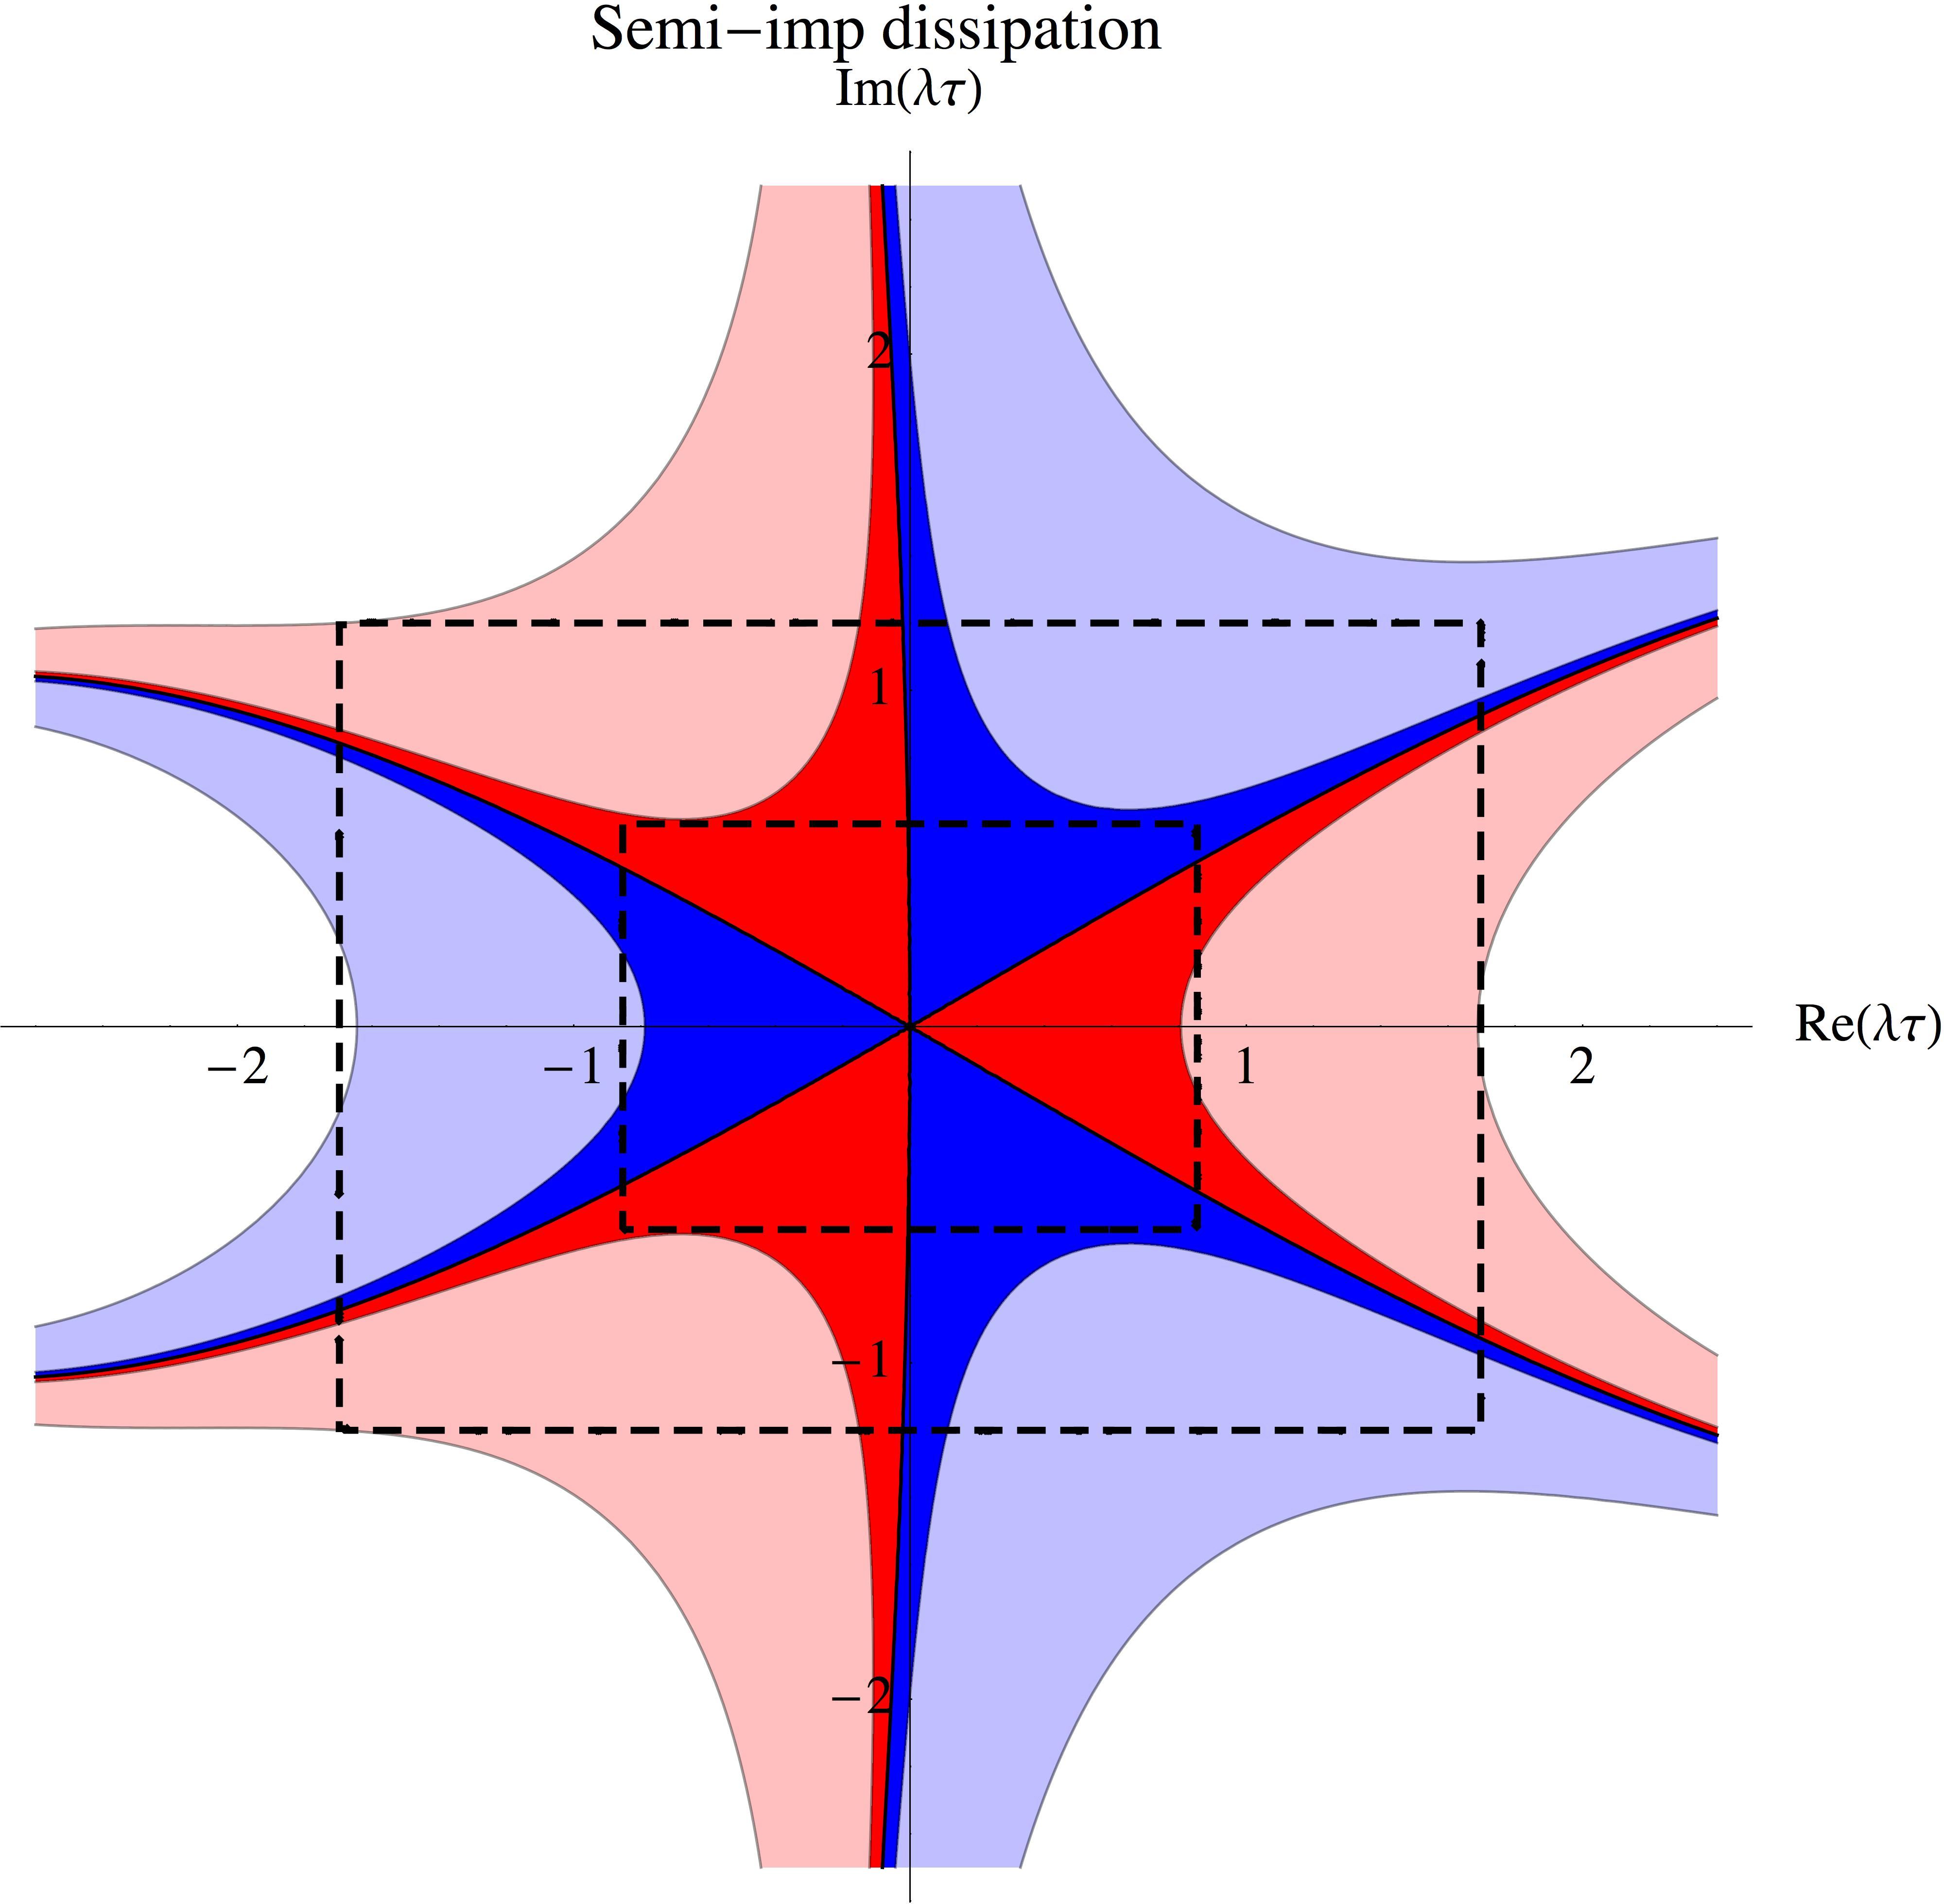
\includegraphics[clip,width=0.49\textwidth]{figs/RK3_imp_diss.jpg}\hfill
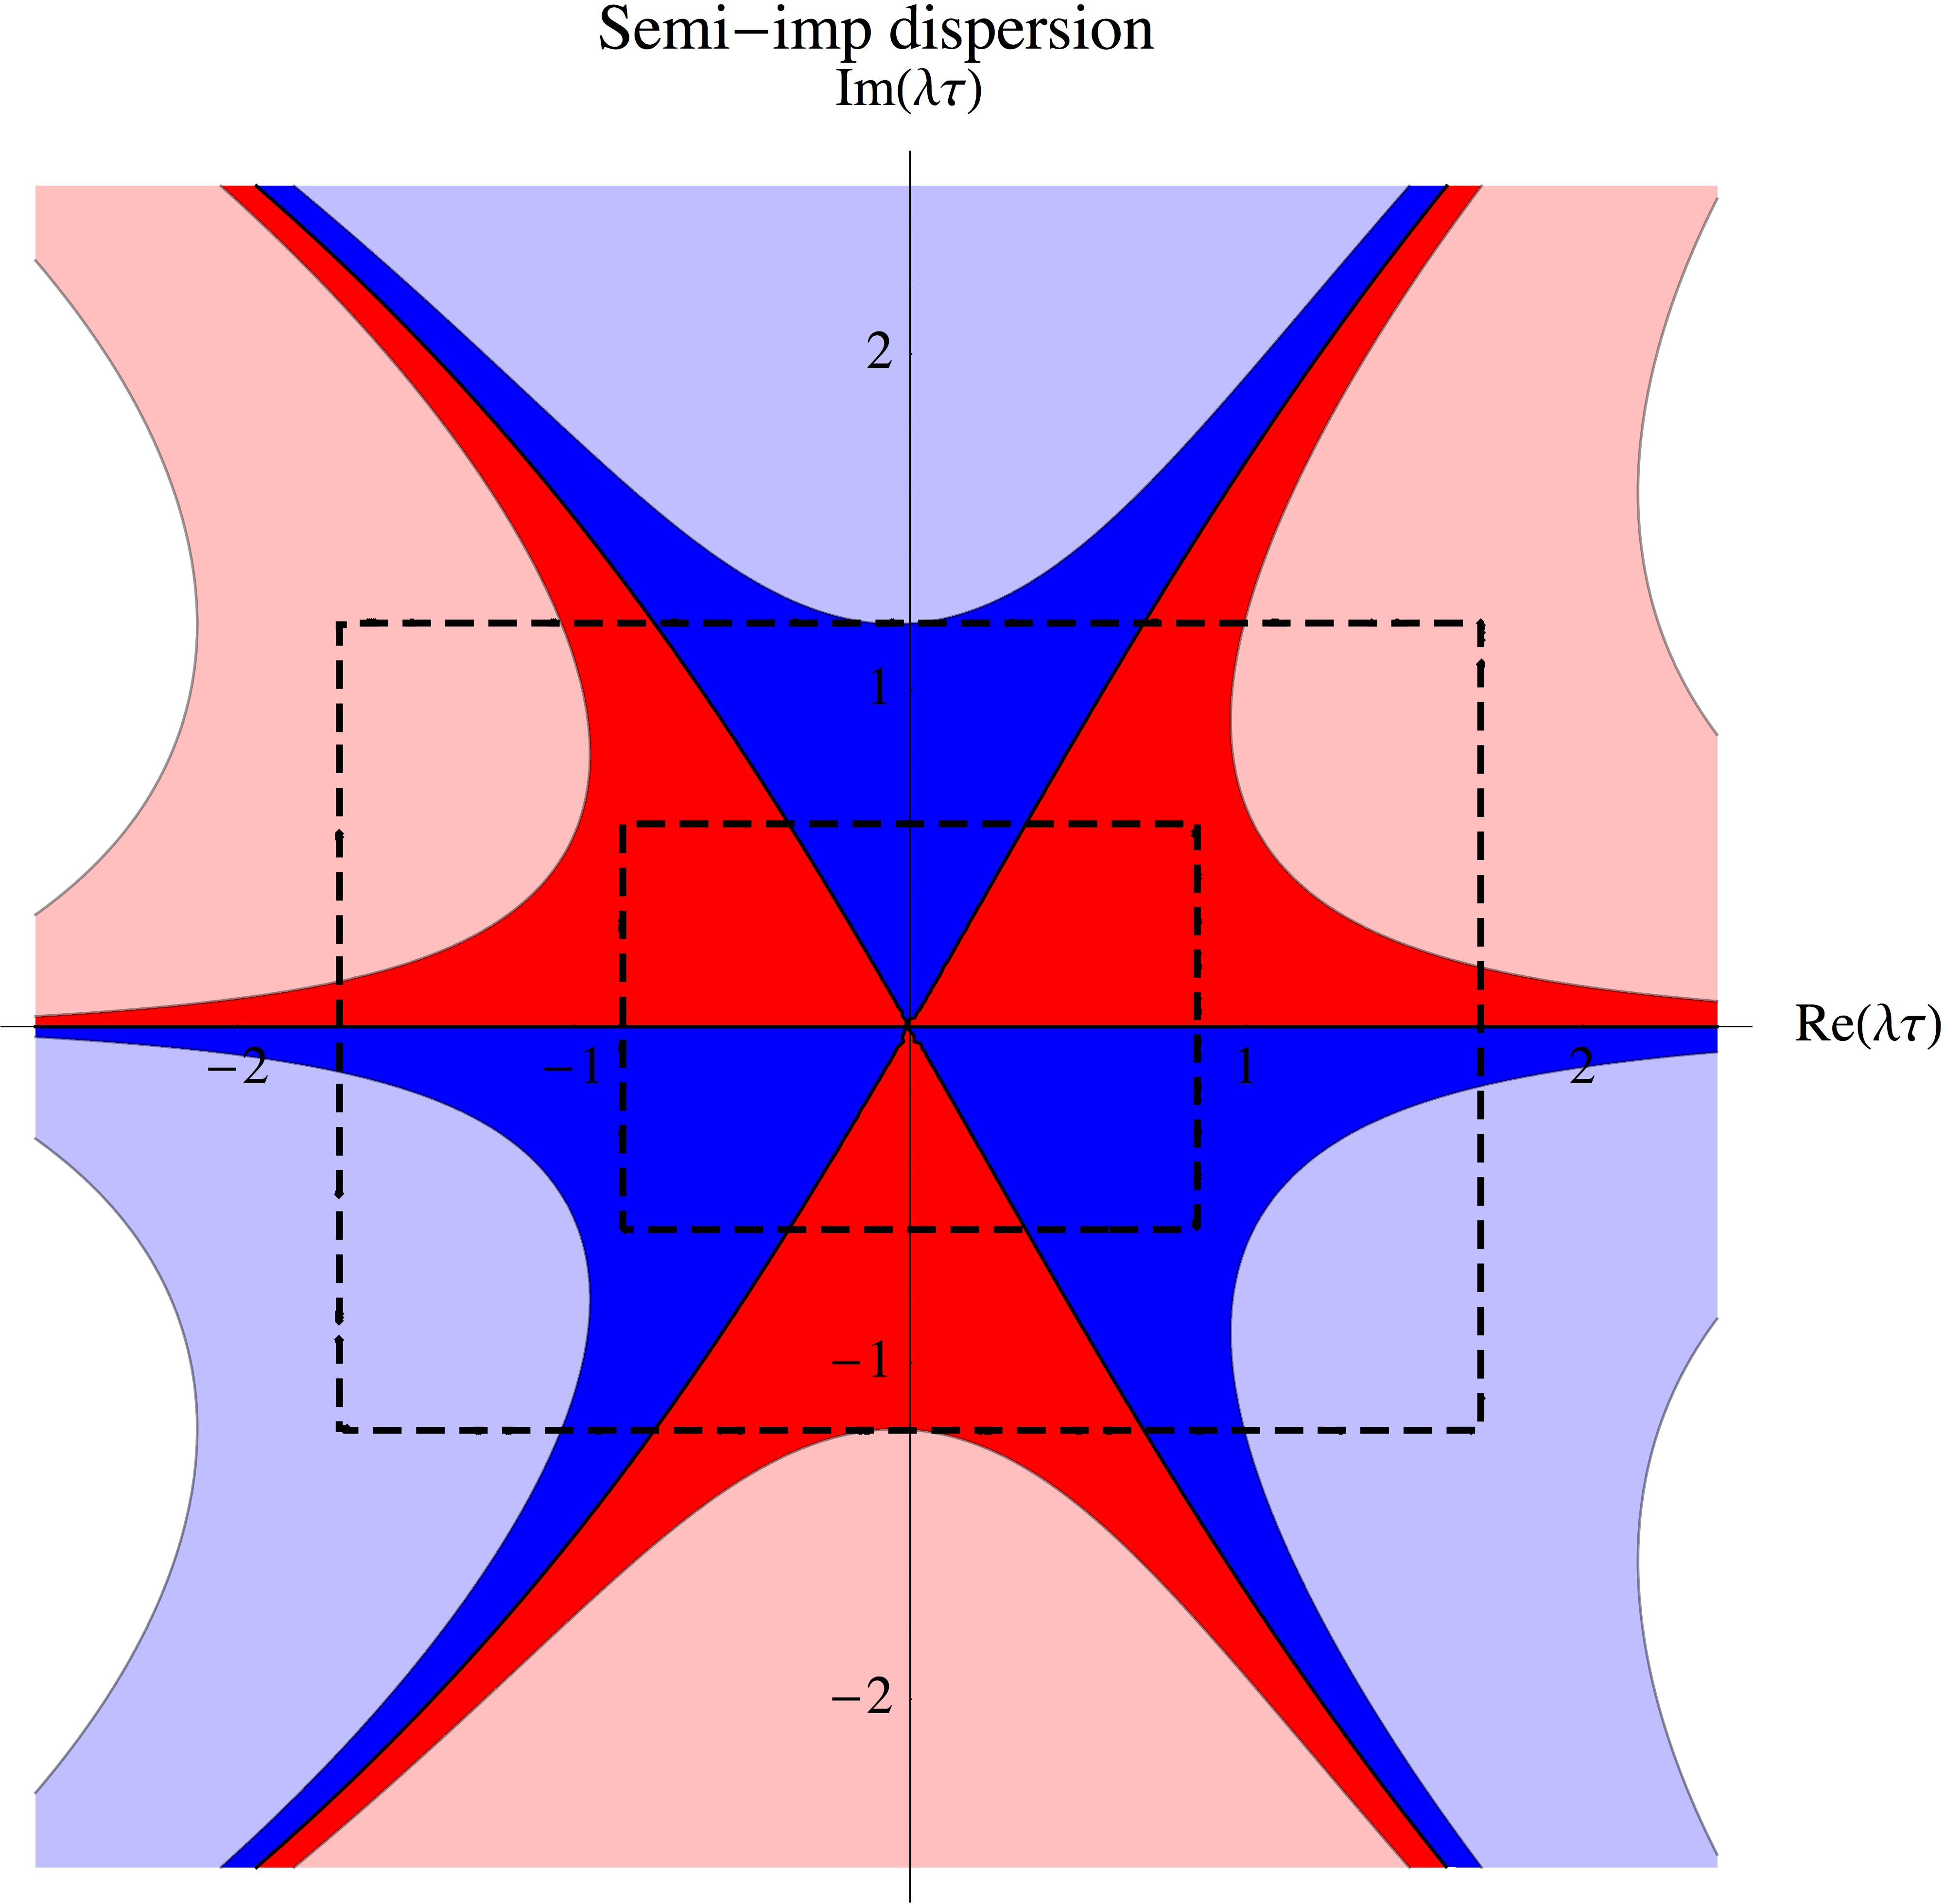
\includegraphics[clip,width=0.49\textwidth]{figs/RK3_imp_disp.jpg}
\caption{Dissipation error (left) associated with the third-order implicit
  Runge-Kutta scheme: dark blue, $0.99<\rho<1$; light blue, $0.90<\rho<0.99$;
  dark red, $1<\rho<1.01$; light red, $1.01<\rho<1.10$. Dispersion error (right)
  associated with the Runge-Kutta scheme: dark blue, $-0.01<\theta/\pi<0$; light
  blue, $-0.10<\theta/\pi<-0.01$; dark red, $0<\theta/\pi<0.01$; light red,
  $0.01<\theta/\pi<0.10$.}\label{fig:rkm3implicit}
\end{figure}
